\documentclass[a4paper]{article}
\usepackage{geometry}
\geometry{left=3.5cm,right=3.5cm,top=3.5cm,bottom=3.5cm}
\usepackage{amsmath, amssymb}
\usepackage{graphicx}
\usepackage{subfigure}
\usepackage{pdfpages}

\usepackage{xeCJK}
\setmainfont{Times New Roman}
\setCJKmainfont[BoldFont=SimHei,ItalicFont=KaiTi]{SimSun}

\usepackage{indentfirst}
\setlength{\parindent}{2em}

\usepackage{fancyhdr}
\pagestyle{fancy}
\usepackage{lastpage}
\rhead{}
\lhead{}
\cfoot{\thepage{}}
\renewcommand{\headrulewidth}{0pt}
\renewcommand{\figurename}{图}
\renewcommand{\tablename}{表}
\renewcommand{\abstractname}{摘要}
\renewcommand{\contentsname}{\CJKfamily{SimHei} 目录}

\headheight 14pt

\usepackage{float}

\renewcommand\baselinestretch{1.2}

\begin{document}

\begin{titlepage}

\includepdf[pages=2-3,offset=0cm 0cm]{title.pdf}

\end{titlepage}

\begin{Huge}
	\centering{\textbf{ATM 交易状态特征分析与异常检测}}
\end{Huge}
\begin{large}
	\begin{flushright}
		
	\end{flushright}
\end{large}
\ \ \\\\

\begin{abstract}
\textit{}
\end{abstract}

\newpage

\tableofcontents

\newpage

\part{引言}
近些年来,由于人民生活水平的提高,银行的业务量飞速提升。与此同时也带了取款存款难的问题。为了解决这个问题,近几年许多银行都开始广泛使用ATM自动取款机,并建立了一套ATM交易系统。但是由于各种原因,ATM交易系统有时会发上故障,影响银行的工作效率。因此,为了实时掌握全行的业务状态,及时发现故障,银行总行数据中心监控系统每分钟会对各分行的交易信息进行汇总统计。汇总信息包括业务量、交易成功率、交易响应时间三个指标。监控系统要从这三个指标的变化情况中及时发现ATM交易系统是否出现故障。本文就如何从这三个指标的变化情况及时发现交易系统的故障做了理论分析,并用所给数据进行了模拟,得到了相对精准的预报。

\part{表征交易状态的特征参量}
ATM交易状态随着时间是不断变化的,但通过观察,我们能够发现ATM交易会有一些固定的模式。而在不同模式下,我们找到了一些特征参量在同一模式下具有稳定性,从而我们可以用这些特征参量来表征ATM交易状态。我们记时间为$t$,业务量为$B(t)$,成功率为S(t),响应时间为R(t)。通过对数据的分析,总的来说,B(t),S(t),R(t)对于时间t大致呈周期分布,且在每一个周期内的不同时间段会显示出不同的模式。因而通过研究每个周期中的不同模式的特征参数,我们便可以了解到ATM交易的模式信息。为了描述这些模式,我们主要通过平均值m,标准差$\sigma$,斜率$\vartheta$这些特征参量来表征不同的状态。同时当有异常值严重偏离我们的特征参数时,我们对于其原因给出了一些分析。下面我们对B(t),S(t),R(t)分别进行分析。
\section{业务量的特征参数}
\indent 对于业务量B(t),通过分析数据,我们将一天划分成四个时段,即:23~次日6点,6~9点,9~18点,18~23点。对于每一个时段,业务量都有一些鲜明的特征。对于23~次日6点,由于是夜间,客户往往不会选择在这段时间办理业务。所以业务量较少,波动不明显,从而$m_B^1$和$\sigma_B^1$都比较小;而6~9点,是业务量上升阶段,这个时段,平均值的意义不是很明显,这里我们用其上升的速度,也即斜率$\vartheta$来表征这一时段的特点;9~18点是一天中业务最为繁忙的一个时期。业务量大,同时波动的幅度也比较明显。所以,这段时间内平均值$m$较大,标准差$\sigma$也很大。第四个时间段是18~23点,这段时间是业务下降阶段。与6~9点类似,我们也用斜率$\vartheta$来记录这一时期的特征。
\indent 业务量是指总行接收到的支行业务总数。当业务量陡然减少时,由于业务量数据是由支行节点通过网络传给总行,所以此时的故障很有可能为支行与总行的网络中断导致的。
\section{成功率的特征参数}
\indent 成功率的模式比较简单,主要分为两个时段。23~次日6这段时间,由于这段时间业务量少,所以银行的通讯线路会非常通畅。但与此同时,也由于业务较少,银行后台要求的稳定性有所降低,同时银行的机器或者程序的检修一般都在晚上进行,从而增大了业务失败的概率,所以这个时间段数据相对比较分散,标准差$\sigma$很大,且有时成功率能达到100\%,有时会很低。另一个时段就是6~23点,这个时期业务量繁多,银行后台的稳定性要求很高,所以这段时间的成功率的标准差比较小。
\indent 影响交易的成功与否的因素很多,比如:分行的数据变更或者配置错误、总行的数据中心后端处理系统应用进程异常等等。若出现上述错误时,就会导致交易成功率下降。所以当成功率出现异常点时,应该及时检查是否这几个地方出现了问题。
\section{响应时间的特征参数}
\indent 响应时间的模式也主要分为两个时段。23~次日6点,由于业务量较少,所以即使响应时间较慢也不会影响银行的处理效率,同时出于降低能耗的原因,银行很有可能会减少夜间服务器的数量,从而使得这期间的响应时间R(t)的平均值较大。而对于6~23点则相反,这段时间业务量巨大,银行必须使用大量的服务器才能满足客户业务量的需求,同时还要尽量减少响应时间以获得更多的业务量。
\indent 响应时间主要受到总行数据中心后台处理系统的影响。当处理系统异常,比如CPU负荷过大时,就会导致交易处理过程缓慢,进而导致响应时间过长。
\section{小结}
通过上面的讨论,我们对这三项指标反应的ATM交易状态特性有了初步的了解,也提取出了每个指标的特征参数。并对每个指标中出现奇异点的原因进行了分析。




\part{交易状态异常检测方案}
\section{基于SSA算法的含噪声时间序列预测}
\section{与其他方法的比较分析}
\section{对方案可靠性的评估}
\section{不同突变点原因分析}

\part{方案的优化及完善}


\end{document}
